% !TeX spellcheck = en_US
\addsection{Introduction}{\spells/magic_arrow.png}

\bigbreak

\hypertarget{Heroes of Might and Magic III}{\textbf{Heroes of Might and Magic III: The Board Game}} is a tactical strategy RPG board game for 1-3 players using the core box set.
The continent of Antagarich is under war as several different Factions, led by their Heroes, battle for supremacy. Choose your Faction and your Hero and banish your unruly enemies from these lands!

\begin{multicols}{2}
\textbf{Notice}: In this rule book, game and component terms are Capitalized.
\textbf{Bold text} is used to draw attention to important rules.
\textit{Italicization} is used for gameplay examples.
\hyperlink{Heroes of Might and Magic III}{Brown colored hyperlinks} refer you to other parts of the rule book.
\vfill
\columnbreak
\note{5}{Exceptions and notes with \hyperlink{Heroes of Might and Magic III}{amber colored hyperlinks} are explained in boxes like this one.}
\vfill
\end{multicols}

\begin{scaledfigure}[blanker]
  \centering
  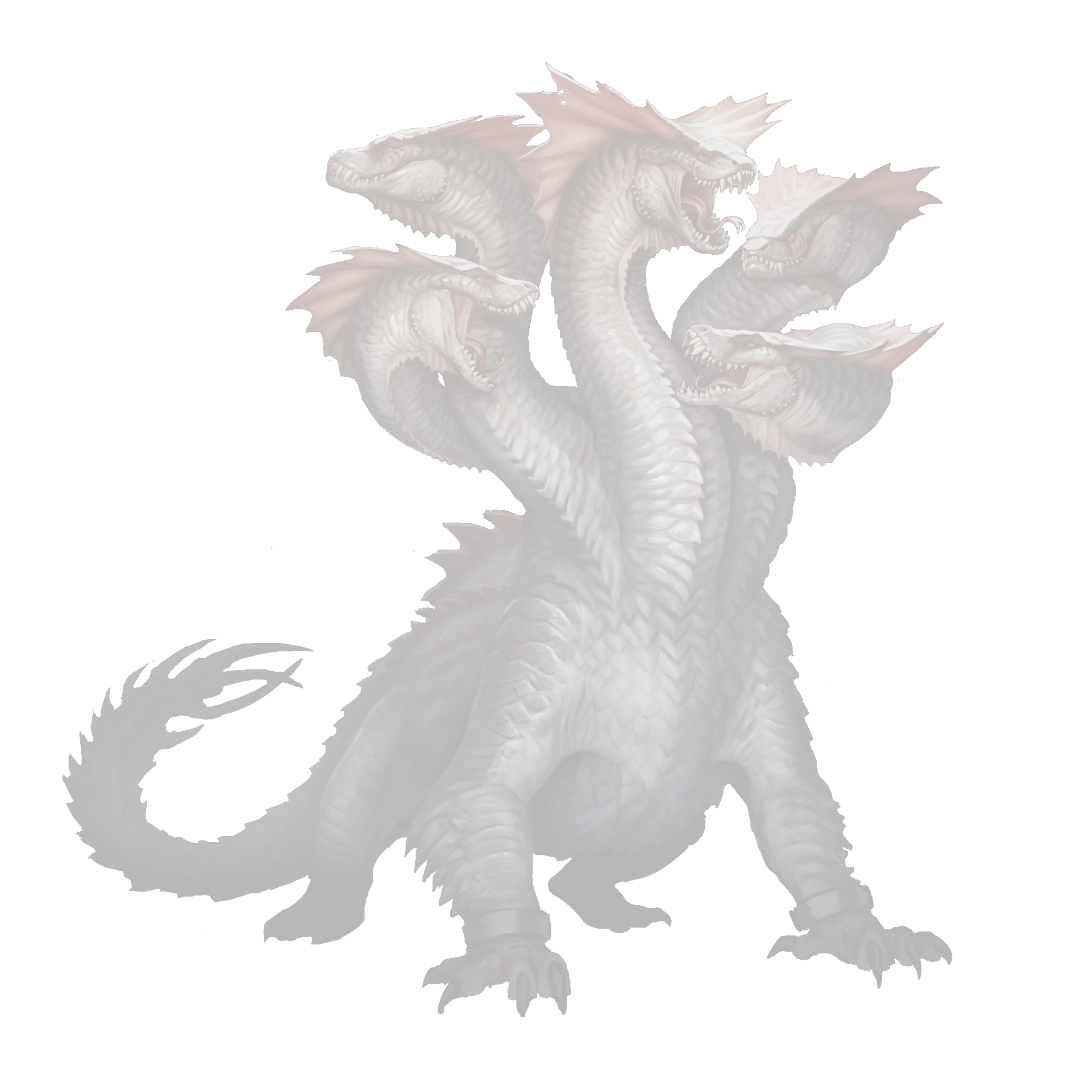
\includegraphics[width=\linewidth, height=\myspace, keepaspectratio]{\art/hydra.png}
\end{scaledfigure}
